\section{Database and selection of test subjects}
\label{Database}
As test samples, a data set of 136 ICAO compliant pictures were given. The data set provided to us is part of the FaceDB database, which  fulfils all parts of our requirements to biometric data sets. In order to get promising morph results, a subset of 10 \todo{number} pairs of photos were selected for manual morphing (\ref{manual_morph}) whereas the automatic morphing algorithm (\ref{automatic_morph}) was applied on different data subsets. For manual  morphing, only pairs with a visually high similarity are considered because the acceptance rate of the comparison algorithm is expected to be higher. 
In sum, 5 manual and 45 automatic morphs are issued in this paper. \footnote{Note that manual morphing is a quite time consuming process and for this reason only a limited amount of manual morphes could be examined.}
\todo[inline]{how many men women?}


\todo[inline]{IN HAUPTTEXT INTEGRIERT: FaceDB}



\subsection{ICAO compliance}
\todo[inline]{DONE ICAO conformance beschrieben}
To fulfil ICAO compliance, a picture has to meet several properties. The whole face should be shown as well as the right and left half. The face, without the hair, should cover 70 - 80 \% of the photo and should be in a centered positon without any rotations. The phote has to be sharp, clear and contrasty in all sections and should be illuminated homogeneously in all passages without reflexions. As background, a single coloured contrasty surface without shadows should be selected. The subject has to look directly into the camera. Especially if the subject wears glasses, reflections should be avoided and the eyes must not be covered by parts of the glasses. The pose should be neutral and the mouth has to be closed. The wearing of headpieces is forbidden but can be permitted e.g. because of religious reasons or long lasting head injuries\cite{bdi2010Verordnung}. 

All photos used in this work are ICAO compliant or nearly ICAO compliant, with respect to the criteria mentioned above. Some of the pictures had the wrong format (the subject was too close to camera). These photos were reformatted to meet the standard with digital post production. It can be ruled out that the post production has any effect on the recognition algorithm. 

\section{Morphing of Faces}
\label{morphing}
The main task during the morphing of two pictures is to detect characteristics and place landmarks as an instruction for the algorithm. This can be done completely automatic or with the support of a user. In this paper both ways are discussed.  
\subsection{Basic idea}
\label{percentageMorph}
For every morph there were 15 images for automatic and 30 for manual created from 0\% of Subject 1 to 100\%, respectively the remaining \% of Person 2. So as an example the 15 images for automatic are combined of:
\begin{itemize}
	\item 1. Picture: Person 1 100\% - Person 2 0\%
	\item 2. Picture: Person 1 92,86\% - Person 2 7,14\%
	\item 3. Picture: Person 1 85,71\% - Person 2 14,29\%
	\item 4. Picture: Person 1 78,57\% - Person 2 21,43\%
	\item 5. Picture: Person 1 71,43\% - Person 2 28,57\%
	\item 6. Picture: Person 1 64,29\% - Person 2 35,71\%
	\item 7. Picture: Person 1 57,14\% - Person 2 42,86\%
	\item 8. Picture: Person 1 50,00\% - Person 2 50,00\%
	\item 9. Picture: Person 1 42,86\% - Person 2 57,14\%
	\item 10. Picture: Person 1 35,71\% - Person 2 64,29\%
	\item 11. Picture: Person 1 28,57\% - Person 2 71,43\%
	\item 12. Picture: Person 1 21,43\% - Person 2 78,57\%
	\item 13. Picture: Person 1 14,29\% - Person 2 85,71\%
	\item 14. Picture: Person 1 7,14\% - Person 2 92,86\%
	\item 15. Picture: Person 1 0\% - Person 2 100\%
	\end{itemize}

\todo[inline]{say something on this + make tabular}
\subsection{Automatic morphing}
\label{automatic_morph}
To generate automatic face morphed images the software FantaMorph 5 was used in this paper. FantaMorph has the ability to create automaticaly morphed faces of to subjects. For this the software defines automatically the landmarks for both faces. These can be adjusted manually by the user afterwards, but in this paper this isn't used. Then the software generates a transition from face 1 to face 2 in a given number of steps, so called frames. For this paper a number of 15/30 steps is used. FantaMorph accepts a list of subjects to which it creates then a sequence to morph from one face to another. It doesn't morph every given subject with every given subject, only from subject 1 to subject 2 and then subejct 2 to subject 3 and so on. So it was not possible to create morphed faces of all subjects instead subsets were created and later on used.\todo{FantaMorph face detection example (2 faces, ein gutes, ein schlechtes)}

\subsubsection{Results}
The resulting morphed sets are 4 different subsets of morphs. The first is the subset of all men sequentially morphed, the second is all women sequentially morphed and the third is all men alternating women sequentially morphed, the last one is the set used from Budrhani.
The number of resulting morphed images are:
\begin{itemize}
	\item Subset 1: 1125 images
	\item Subset 2: 885 images
	\item Subset 3: 1800 images
	\item Subset 4: 225 images
\end{itemize}


\subsection{Manual morphing}
\label{manual_morph}
\begin{figure}[h]
	\centering
	\subfloat[Subject 1]{%
		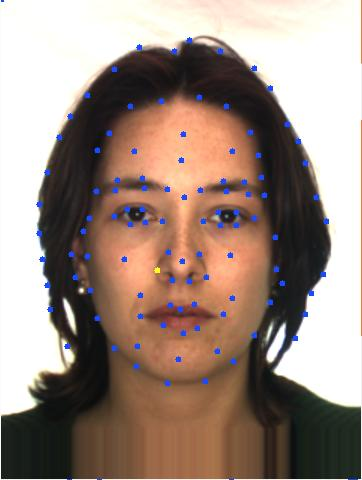
\includegraphics[width=0.25\linewidth]{Resources/manualmorph01.jpg}}
	\label{subfig:manualmorph01}\hspace{10pt}
	\subfloat[Morph no. 5]{%
		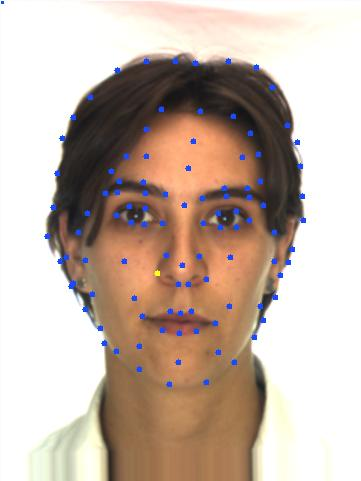
\includegraphics[width=0.25\linewidth]{Resources/manualmorph02.jpg}}
	\label{subfig:manualmorph02}\\
	\caption{Example of two ICAO compliant photos with manually set and shifted landmarks.}
	\label{fig:manual_morph} 
\end{figure}
In contrast to the automatic face morphing approach, manual morphing is discussed in this section. 

To achieve morphes, the open source software GNU Image Manipulation Software (GIMP) (Version 2.8.16) with the GIMP Animation Package (GAP) (Version 2.6) was selected. Morphing with GAP follows the simple approach of manually placing connected landmarks at characterizing points in both faces. In \autoref{fig:manual_morph}, two pictures with a setup of landmarks are shown. It can be observed that the landmarks are placed at characterizing points in both faces, e.g. at the eye browns, lips and nose. The general shape of the face as well as the shape of the head, including the hair, is also respected. In the example, the facial landmarks are close to each other, whereas the landmarks describing the shape of the hair are further apart. 

The selection of characterizing points \todo{regions?} is based on findings \todo{erkenntnissen?} from earlier works on the topic of automatic face recognition, to achieve an optimal morphing result compared with own estimation based on the individual appearance of the subjects. \cite[60ff]{jain2008handbook} \cite{amos2016openface} \todo{DONE cite handbook of bio p.60} \todo{cite these fancy mp4 thingy}.
The algorithm shifts the landmarks from face one to face two. In addition to this, the colour of the skin is transmitted. 

%\subsubsection*{Morphing setup}
For the test samples 100 - 125 landmarks were placed, depending on the face characteristics. The output contains a sequence of 30 photos which show different stages of the morphing procedure. \ref{1e}


\subsubsection{Results}
\todo{compare to automatic results when there.}
\begin{figure}[h]
	\centering
	\subfloat[Subject 1]{%
		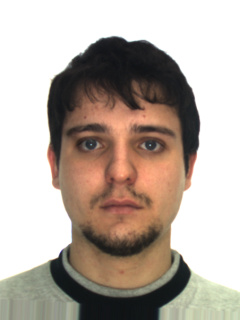
\includegraphics[width=0.19\linewidth]{Resources/p1.jpg}
	\label{1a}}\hfill
	\subfloat[Morph no. 5]{%
		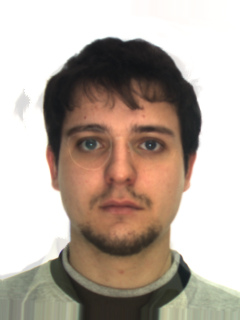
\includegraphics[width=0.19\linewidth]{Resources/m1.jpg}
	\label{1b}}\hfill
	\subfloat[Morph no. 15]{%
		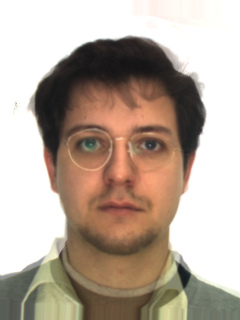
\includegraphics[width=0.19\linewidth]{Resources/m2.jpg}
	\label{foo}} \hfill
	\subfloat[Morph no. 25]{%
		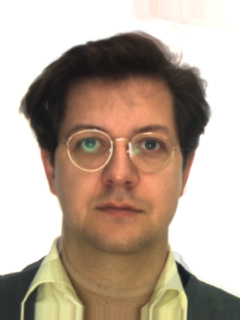
\includegraphics[width=0.19\linewidth]{Resources/m3.jpg}
	\label{1d}}\hfill
	\subfloat[Subject 2]{%
		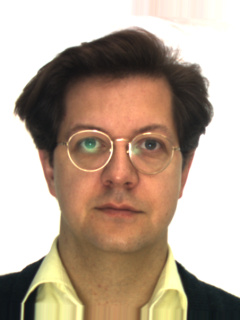
\includegraphics[width=0.19\linewidth]{Resources/p2.jpg}
	\label{1e} }
	\caption{Example of two ICAO compliant photos (\ref{1a} and \ref{1e}) and morphs at stage 5 (\ref{1b}), 15 (\ref{foo}) and 25 (\ref{1d})}
	\label{fig1} 
\end{figure}

In figure \ref{fig1} a two subjects and three morphing stages (5, 15 and 25) are shown. The visual inspection of \ref{1a} shows biometric features of both subjects whereas \subref{1e} and \ref{1d} have more similarity to the closer subject but also covers features of the other subject.
A manual post production of the morphs is not necessary because potential revealing details, like the interference \todo{?} of the clothes, glasses or hair is not considered by the algorithm.

\todo[inline]{OK Detailed description of the morphs}
